\section{Introduction}
Nursery scouting from unmanned aerial vehicles (UAVs) is a high-resolution, small-object problem. A single RGB frame may contain many repeated plants, uneven spacing, partial crowns, shadows, ground fabric, and row-edge truncation. Conventional detectors can localize and count annotated instances, but their output does not directly express scouting state, confidence, or the need for human review. General-purpose VLMs provide a richer interface, yet whole-image inference is poorly matched to 5K aerial imagery: downsampling erases small instances, exhaustive tiling is expensive, and free-form responses can remain syntactically valid while being visually unsupported. Prior edge-deployed UAV systems further motivate bounded inference when sensing and control must operate under finite onboard resources~\cite{kode2026drone}.

This work studies a narrower and falsifiable problem. Given a fixed budget of VLM calls per source image, can detector evidence identify informative regions, and can a validation-calibrated gate reduce unsupported compact-VLM decisions when the crop changes? The distinction matters. The detector supplies localized evidence; the VLM is responsible for a constrained semantic record; and the gate decides whether that record is reliable enough to use. None of these components is treated as an agronomic authority.

The evaluation uses two visually and geometrically different ornamental crops, Magnolia and Azalea. The relabeled corpus contains 297 Magnolia and 121 Azalea source images, with 15,644 and 14,198 usable boxes, respectively. Azalea has a higher median instance count (97 versus 57 plants per image) and a 44.1\% smaller median normalized box area. The crops also differ in greenness and spatial arrangement. We therefore treat crop identity as a domain shift rather than randomly mixing all tiles before splitting.

Our contributions are:
\begin{itemize}[leftmargin=*,nosep]
    \item a Budgeted Evidence Selector for high-resolution aerial imagery that combines detector confidence and clipped local count while preserving an explicit exploration fraction;
    \item a structured compact-VLM scouting task with hard-negative evaluation, repeated-generation consistency, and schema-level failure measurements;
    \item a validation-only selective gate evaluated through risk--coverage analysis rather than a single confidence threshold; and
    \item a source-safe cross-crop protocol with clustered confidence intervals, transfer matrices, edge-oriented latency and memory measurements, and equal-budget ablations.
\end{itemize}

The intended claim is algorithmic, not merely agricultural: localized evidence should be used to allocate scarce multimodal computation, and unsupported outputs should be reviewable rather than silently accepted.

\begin{figure*}[t]
    \centering
    \resizebox{\textwidth}{!}{\begin{tikzpicture}[
  font=\sffamily\scriptsize,
  box/.style={draw=black!68, rounded corners=1.2pt, align=center,
    minimum height=9mm, text width=22mm, inner sep=2.5pt},
  compact/.style={box, text width=19mm, minimum height=8mm, inner sep=2pt},
  data/.style={box, fill=blue!5},
  prep/.style={box, fill=cyan!7},
  evidence/.style={box, fill=green!7},
  select/.style={compact, fill=orange!10, draw=orange!72!black},
  vlm/.style={box, fill=violet!7, draw=violet!62!black},
  reliable/.style={box, fill=teal!8, draw=teal!65!black},
  outputbox/.style={compact, fill=gray!6},
  sample/.style={draw=black!70, line width=.45pt, inner sep=0pt, fill=white},
  stage/.style={draw=black!45, dashed, rounded corners=2pt,
    inner xsep=1.4mm, inner ysep=2.5mm},
  flow/.style={-{Latex[length=1.9mm,width=1.35mm]}, line width=.7pt, draw=black!78},
  train/.style={flow,dashed, draw=black!58},
  junction/.style={circle, fill=black!78, inner sep=0pt, minimum size=1.15mm}
]

% Row 1: real cross-crop inputs, source-safe preparation, and local evidence.
\node[sample] (magback) {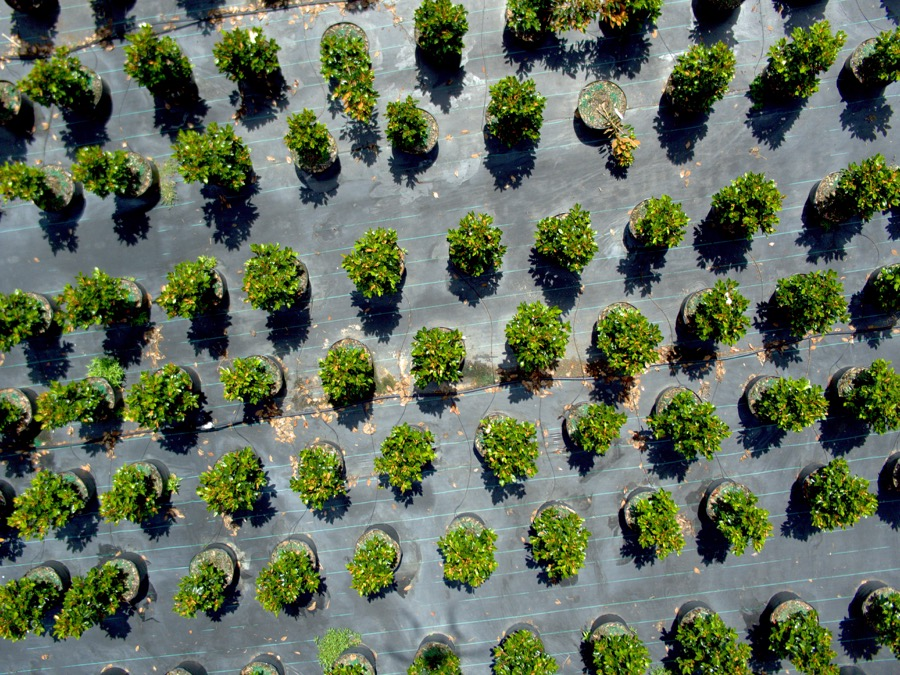
\includegraphics[width=20mm,height=15mm]{figures/input_examples/magnolia_03.jpg}};
\node[sample, xshift=-1.6mm, yshift=1.4mm] at (magback.center) (magmid)
  {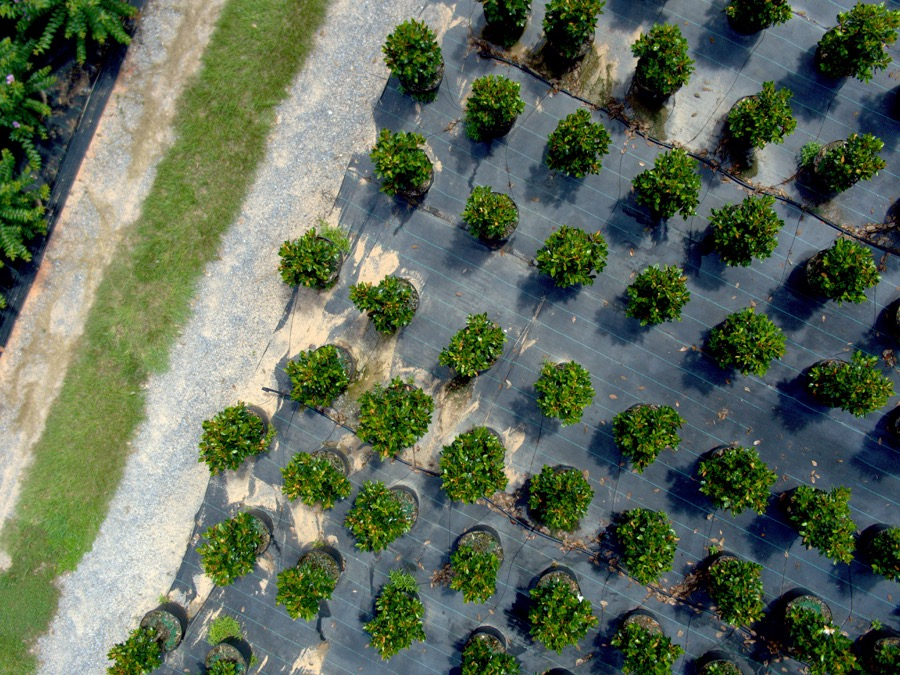
\includegraphics[width=20mm,height=15mm]{figures/input_examples/magnolia_02.jpg}};
\node[sample, xshift=-1.6mm, yshift=1.4mm] at (magmid.center) (mag)
  {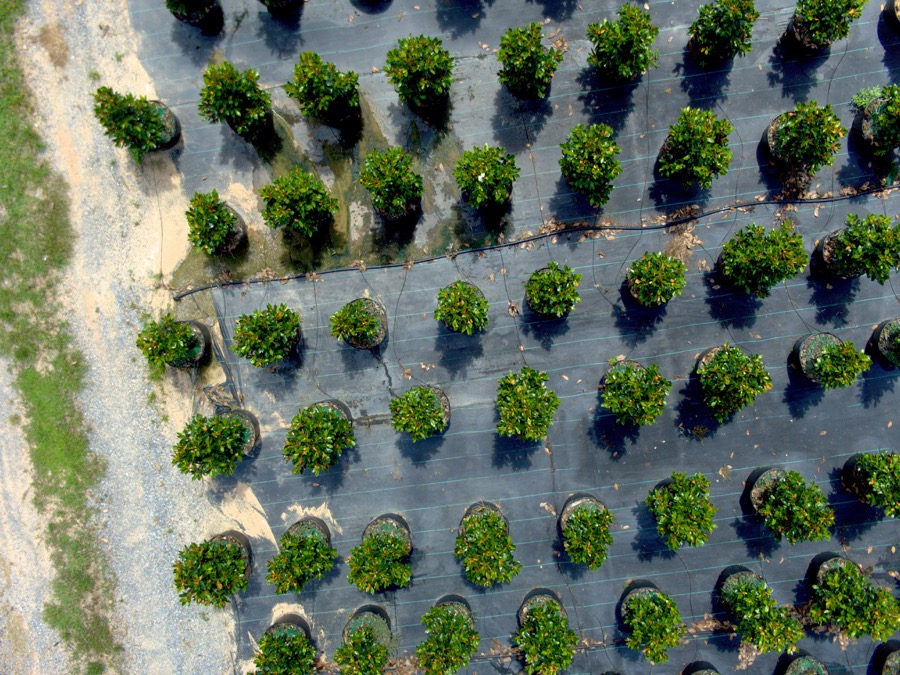
\includegraphics[width=20mm,height=15mm]{figures/input_examples/magnolia_01.jpg}};
\node[fit=(magback)(magmid)(mag), inner sep=.4mm] (magstack) {};
\node[font=\bfseries\scriptsize, above=.7mm of magstack] (maglabel) {Magnolia RGB};

\node[sample, below=8mm of magback] (azaback)
  {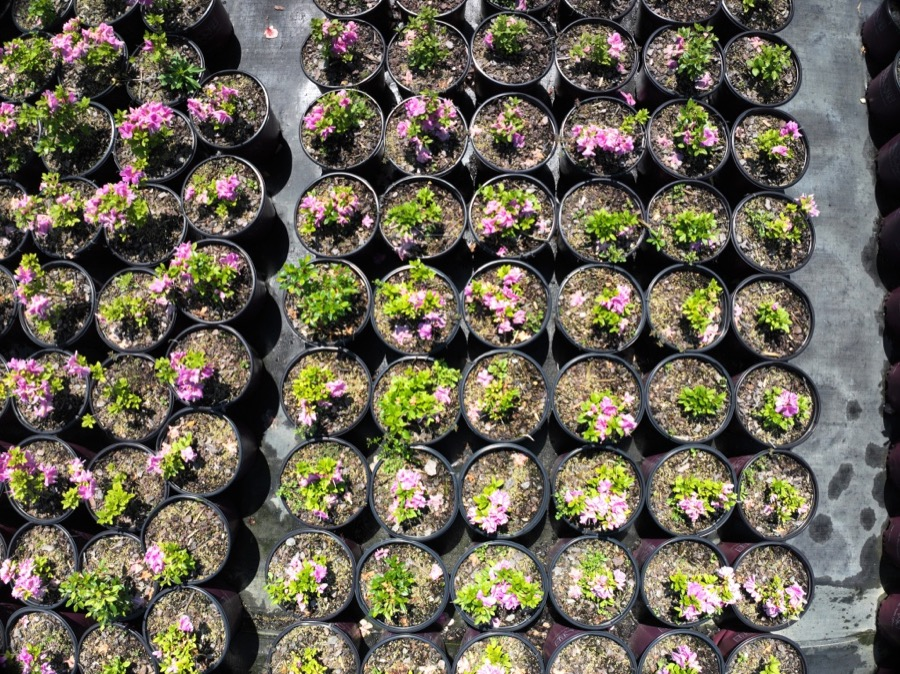
\includegraphics[width=20mm,height=15mm]{figures/input_examples/azalea_03.jpg}};
\node[sample, xshift=-1.6mm, yshift=1.4mm] at (azaback.center) (azamid)
  {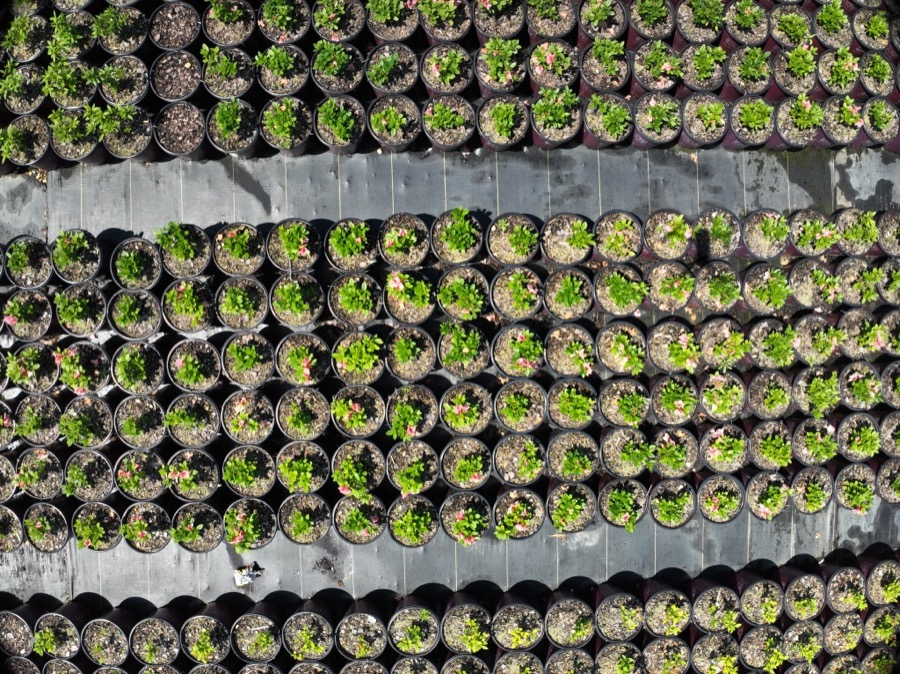
\includegraphics[width=20mm,height=15mm]{figures/input_examples/azalea_02.jpg}};
\node[sample, xshift=-1.6mm, yshift=1.4mm] at (azamid.center) (aza)
  {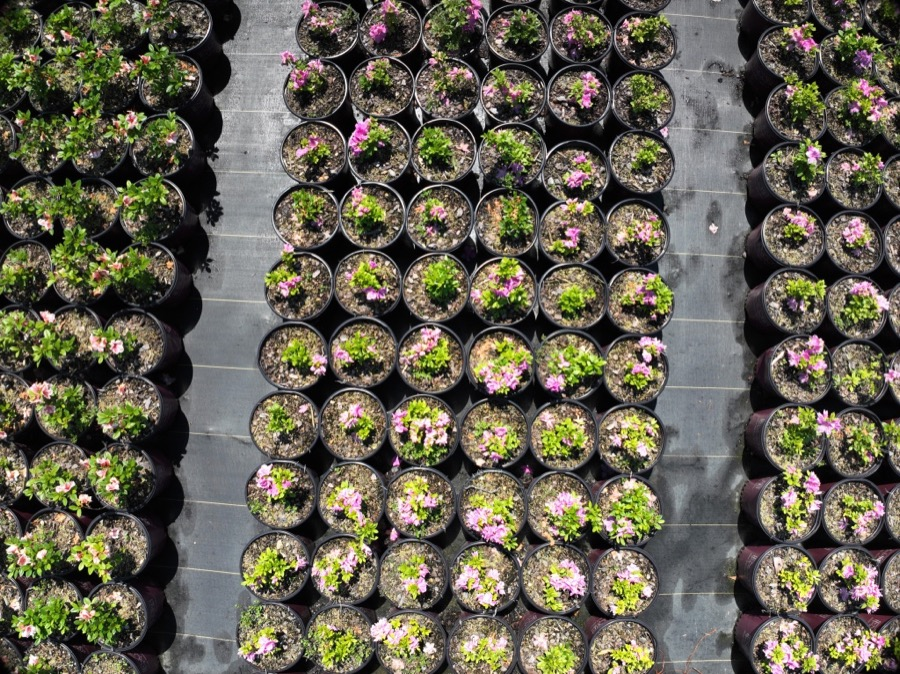
\includegraphics[width=20mm,height=15mm]{figures/input_examples/azalea_01.jpg}};
\node[fit=(azaback)(azamid)(aza), inner sep=.4mm] (azastack) {};
\node[font=\bfseries\scriptsize, above=.7mm of azastack] (azalabel) {Azalea RGB};

\node[prep, right=6mm of $(magstack.east)!0.5!(azastack.east)$] (split)
  {\textbf{Source split}\\train / val / test\\before tiling};
\node[prep, right=5mm of split] (tile)
  {\textbf{Overlapping tiles}\\$s\!\times\!s$, overlap $\alpha$};
\node[evidence, right=5mm of tile] (det)
  {\textbf{Detector evidence}\\confidence $c_t$\\count $n_t$};
\node[outputbox, right=5mm of det, fill=yellow!12, draw=orange!68!black] (labels)
  {\textbf{One-class boxes}\\training / scoring only};

% Row 2: selector, structured inference, and selective output.
\node[select, below=11mm of azastack] (rank)
  {\textbf{Evidence rank}\\$q_t=c_t+\bar n_t$};
\node[select, right=4mm of rank] (allocate)
  {\textbf{Allocate}\\top $K_x$ + explore $K_e$};
\node[select, right=4mm of allocate] (union)
  {\textbf{Budget union}\\$|\mathcal{S}_i|\leq K$};
\node[vlm, right=6mm of union] (adapter)
  {\textbf{VLM adapter}\\SmolVLM2 / Phi\\LLaVA};
\node[vlm, right=4mm of adapter] (schema)
  {\textbf{Schema decoder}\\fixed fields; no\\silent repair};
\node[reliable, right=5mm of schema] (signals)
  {\textbf{Reliability evidence}\\schema, repeats,\\detector agreement};
\node[reliable, right=4mm of signals] (gate)
  {\textbf{Failure-risk gate}\\validation-fitted\\threshold $\tau^*$};
\node[outputbox, right=4mm of gate, fill=green!8, draw=green!55!black] (accept)
  {\textbf{Accept}\\retain record};
\node[outputbox, below=3mm of accept, fill=orange!9, draw=orange!68!black] (review)
  {\textbf{Review}\\abstain / inspect};
\node[outputbox, below=5mm of gate, text width=22mm] (val)
  {\textbf{Validation outcomes}\\observed task failures};

% Boundary-to-boundary paths.
\draw[flow] (magstack.east) -- ++(1.4mm,0) |- ($(split.west)+(0,2mm)$);
\draw[flow] (azastack.east) -- ++(3.0mm,0) |- ($(split.west)+(0,-2mm)$);
\draw[flow] (split.east) -- (tile.west);
\draw[flow] (tile.east) -- (det.west);
\draw[train] (labels.west) -- (det.east);
\coordinate (selectorlane) at ($(rank.north)+(0,2.2mm)$);
\draw[flow] (det.south) |- (selectorlane) -- (rank.north);
\draw[flow] (rank.east) -- (allocate.west);
\draw[flow] (allocate.east) -- (union.west);
\draw[flow] (union.east) -- (adapter.west);
\draw[flow] (adapter.east) -- (schema.west);
\draw[flow] (schema.east) -- (signals.west);
\draw[flow] (signals.east) -- (gate.west);
\node[junction] (gatebranch) at ($(gate.east)+(2mm,0)$) {};
\draw[line width=.7pt, draw=black!78] (gate.east) -- (gatebranch);
\draw[flow] (gatebranch) -- (accept.west);
\draw[flow] (gatebranch) |- (review.west);
\draw[train] (val.north) -- node[right,font=\tiny]{fit on val only} (gate.south);

\begin{scope}[on background layer]
  \node[stage, fit=(maglabel)(magstack)(azalabel)(azastack)(split)(tile)] (stageA) {};
  \node[stage, fit=(det)(labels)] (stageB) {};
  \node[stage, fit=(rank)(allocate)(union), draw=orange!72!black] (stageC) {};
  \node[stage, fit=(adapter)(schema), draw=violet!55!black] (stageD) {};
  \node[stage, fit=(signals)(gate)(accept)(review)(val), draw=teal!55!black] (stageE) {};
\end{scope}

% Stage headings are independent of the dashed frames so text never touches a boundary.
\node[font=\bfseries\scriptsize, above=1.1mm of stageA.north]
  {A. Source-safe preparation};
\node[font=\bfseries\scriptsize, above=1.1mm of stageB.north]
  {B. Local evidence};
\node[font=\bfseries\scriptsize, text=orange!55!black, below=1.1mm of stageC.south]
  {C. Budgeted Evidence Selector};
\node[font=\bfseries\scriptsize, text=violet!40!black, below=1.1mm of stageD.south]
  {D. Structured VLM inference};
\node[font=\bfseries\scriptsize, text=teal!38!black, above=1.1mm of stageE.north]
  {E. Selective reliability};
\end{tikzpicture}
}
    \caption{\textbf{OrnaScout overview.} Source images are partitioned before tiling. Detector confidence and clipped local count rank candidate tiles; the proposed selector combines top-ranked exploitation with controlled exploration under a fixed budget $K$. A model adapter and fixed-schema decoder produce auditable task records. Reliability signals enter a failure-risk gate fitted only on validation outcomes; accepted records are retained and the remainder are referred for review. Solid arrows denote test-time computation and dashed arrows denote supervision or validation-only fitting.}
    \label{fig:architecture}
\end{figure*}
